\chapter*{Anexo B: Publicación en HCOMP 2017}
\label{anexo:paper}

Durante el periodo de desarrollo de esta tesis se aceptó una publicación sobre el sistema de detección de sismos propuesto y su evaluación en \textit{The 5th AAAI Conference on Human Computation and Crowdsourcing} (HCOMP 2017)

Esta conferencia se encarga de difundir los últimos descubrimientos de investigaciones relacionadas con \textit{crowdsourcing} y \textit{human computation}. En este evento también se presentan muchos estudios relacionados con interacción humano computador (HCI), inteligencia artificial y muchos de ellos corresponden a trabajos interdiciplinarios. Parte del trabajo propuesto en esta tesis tiene las características necesarias para ser considerada dentro del área de investigación de \textit{Natural Human Computation}, un tipo de \textit{Human Computation} que busca obtener conocimiento a partir del comportamiento de las personas extrayendo trabajo computacional significativo sin perturbar su comportamiento normal~\cite{EstradaAndLawhead}. 

También se vivió la experiencia de presentar en la conferencia sobre el trabajo realizado frente a un público internacional.

\begin{figure}[!h]
\centering
	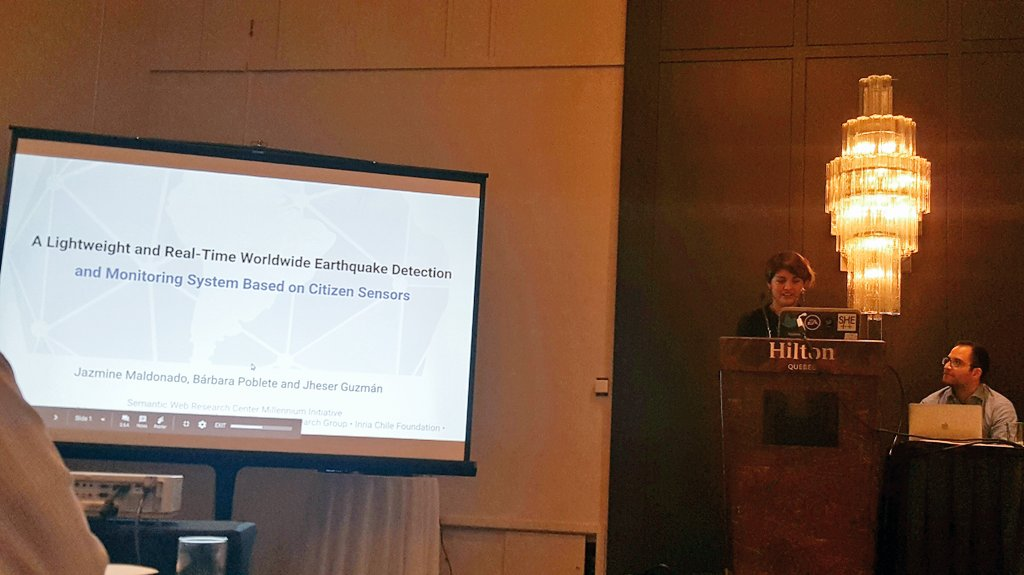
\includegraphics[width=0.5\textwidth]{imagenes/hcomp.jpg}
	\caption{Jazmine Maldonado presentando en HCOMP 2017.}
\label{fig:hcomp}
\end{figure} 

El artículo publicado se adjunta en la siguiente página. 

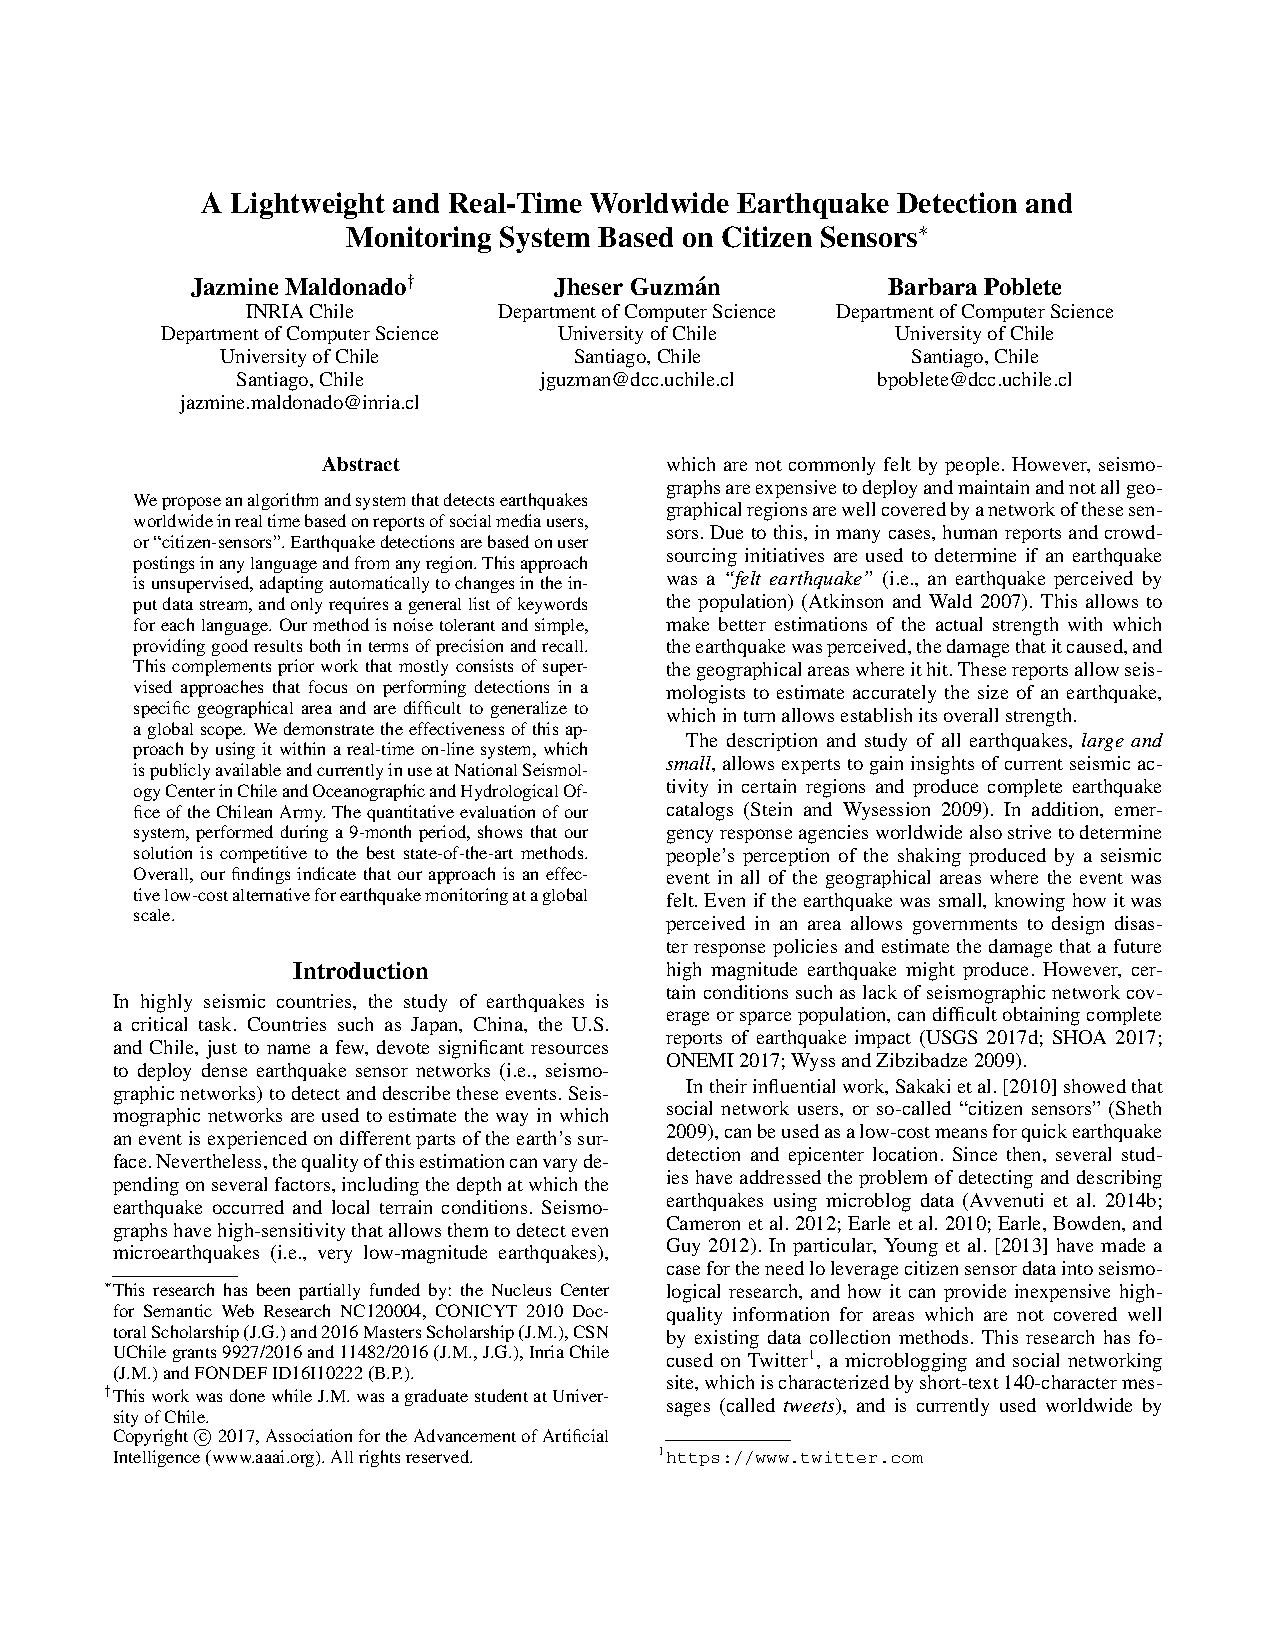
\includepdf[pages={1-10},scale=1]{documentos/paper_earthquake.pdf}